% =====================================================================
% THIS FILE IS THE SOURCE. Edit it, then rebuild the PDF with:
%     bash tools/compile.sh Unit_01_Inference
% (run from the Course_Rewrite folder; it compiles twice and reports
%  page count, overfull boxes, and em dashes)
%
% Do not edit the PDF directly. Figures are the fig_*.pdf files in this
% folder, regenerated by tools/make_module*_slide_figs.py.
%
% Originally converted from the 15-module draft by a one-shot script now
% parked in tools/one_shot_generators/. Re-running those would discard
% anything you change here, so they are kept out of tools/ on purpose.
% =====================================================================
\documentclass[aspectratio=169]{beamer}
\usetheme{default}
\usefonttheme{professionalfonts}
\usepackage{amsmath, amssymb, amsfonts}
\usepackage{graphicx}
\usepackage{booktabs}
\usepackage{bm}
\usepackage{hyperref}

\mode<presentation> {
    \usetheme{Frankfurt}
    \usecolortheme{default}
}

% == notation shortcuts ==
\newcommand{\xbar}{\bar{x}}
\newcommand{\SE}{\mathrm{SE}}
\newcommand{\se}{\widehat{\SE}}
\newcommand{\E}{\mathbb{E}}
\newcommand{\Hzero}{H_0}
\newcommand{\Hone}{H_1}

% Recurring motifs (color-coded). Frankfurt: block=blue, alert=red, example=green.
\newenvironment{principle}[1]{\begin{block}{\textbf{Principle:} #1}}{\end{block}}
\newenvironment{trap}[1]{\begin{alertblock}{\textbf{Trap:} #1}}{\end{alertblock}}
% Green block, used two ways: a worked judgment call, or (sparingly) a question
% you should be ready to field out loud.
\newenvironment{practice}[1]{\begin{exampleblock}{\textbf{In practice:} #1}}{\end{exampleblock}}
\newenvironment{interview}[1]{\begin{exampleblock}{\textbf{You may be asked:} #1}}{\end{exampleblock}}
% "Your turn" pause-and-answer prompt (orange, locally colored).
\newenvironment{yourturn}[1]{%
  \setbeamercolor{block title}{fg=white,bg=orange!80!black}%
  \setbeamercolor{block body}{bg=orange!12}%
  \begin{block}{\textbf{Your turn:} #1}}{\end{block}}
% "Live demo" prompt (teal, locally colored).
\newenvironment{livedemo}[1]{%
  \setbeamercolor{block title}{fg=white,bg=teal!80!black}%
  \setbeamercolor{block body}{bg=teal!12}%
  \begin{block}{\textbf{Live demo:} #1}}{\end{block}}
% "LLM check" prompt (violet, locally colored).
\newenvironment{llmcheck}[1]{%
  \setbeamercolor{block title}{fg=white,bg=violet!75!black}%
  \setbeamercolor{block body}{bg=violet!10}%
  \begin{block}{\textbf{LLM check:} #1}}{\end{block}}

\title{Statistical Inference}
\subtitle{Unit 1: Signal, Noise, and What a Test \emph{Really} Tells You}
\author{Stat 220 \textbar{} Statistics for Data Science}
\date{}

\begin{document}

\begin{frame}
  \titlepage
\end{frame}

% ======================================================================
\section{Why}
% ======================================================================
\begin{frame}{What this course is actually about}
\begin{itemize}
  \item Running a statistical test is free. Any library hands you a $t$-statistic and a
        $p$-value in milliseconds, and it will do it just as fast when the answer is garbage.
  \item The hard part is knowing what the number means \emph{here}, in this messy situation,
        with this data, for this decision.
  \item So the question we keep coming back to all semester is not ``what is the $p$-value?''
        It is: \textbf{what would this look like if nothing were going on?}
\end{itemize}
\vspace{0.4em}
\centering\small
Let's start by running an experiment on ourselves.
\end{frame}

% == OPENING LIVE ACTIVITY (before any theory, before Fisher) ==
\begin{frame}{Review: the one-sample $t$-test, all on one page}
\footnotesize
You have one sample and a claimed value $\mu_0$. Steps: state the hypotheses, compute
$t$, compare, report.
\[
t \;=\; \frac{\xbar - \mu_0}{s/\sqrt{n}}, \qquad \text{df} = n-1 .
\]
\begin{center}
\begin{tabular}{p{0.20\textwidth} p{0.24\textwidth} p{0.21\textwidth} p{0.22\textwidth}}
\toprule
\textbf{Alternative} & \textbf{Use when you care about} & \textbf{Reject $\Hzero$ when}
& \textbf{$p$-value} \\
\midrule
$\Hone:\ \mu > \mu_0$ \newline (right-tailed) & only an increase counts
& $t > t_{\alpha,\,df}$ & $\Pr(T \ge t)$ \\[4pt]
$\Hone:\ \mu < \mu_0$ \newline (left-tailed) & only a decrease counts
& $t < -t_{\alpha,\,df}$ & $\Pr(T \le t)$ \\[4pt]
$\Hone:\ \mu \neq \mu_0$ \newline (two-tailed) & a change in either direction
& $|t| > t_{\alpha/2,\,df}$ & $2\Pr(T \ge |t|)$ \\
\bottomrule
\end{tabular}
\end{center}
\vspace{0.2em}
\begin{trap}{choose the side before you see the data}
A one-tailed test is easier to pass, so picking the direction after looking at the result doubles
your real false-positive rate. If you would have been interested in a move either way, it is
two-tailed.
\end{trap}
\end{frame}

\begin{frame}{Live experiment: find a Coke expert}
\vfill
\begin{livedemo}{I need a volunteer}
\centering
\Large Someone who is \textbf{sure} they can taste the difference between
\textbf{Coke} and \textbf{Coke Zero}.
\end{livedemo}
\vfill
\end{frame}

\begin{frame}{What ``just guessing'' actually looks like}
\begin{columns}[c]
\begin{column}{0.66\textwidth}
\centering
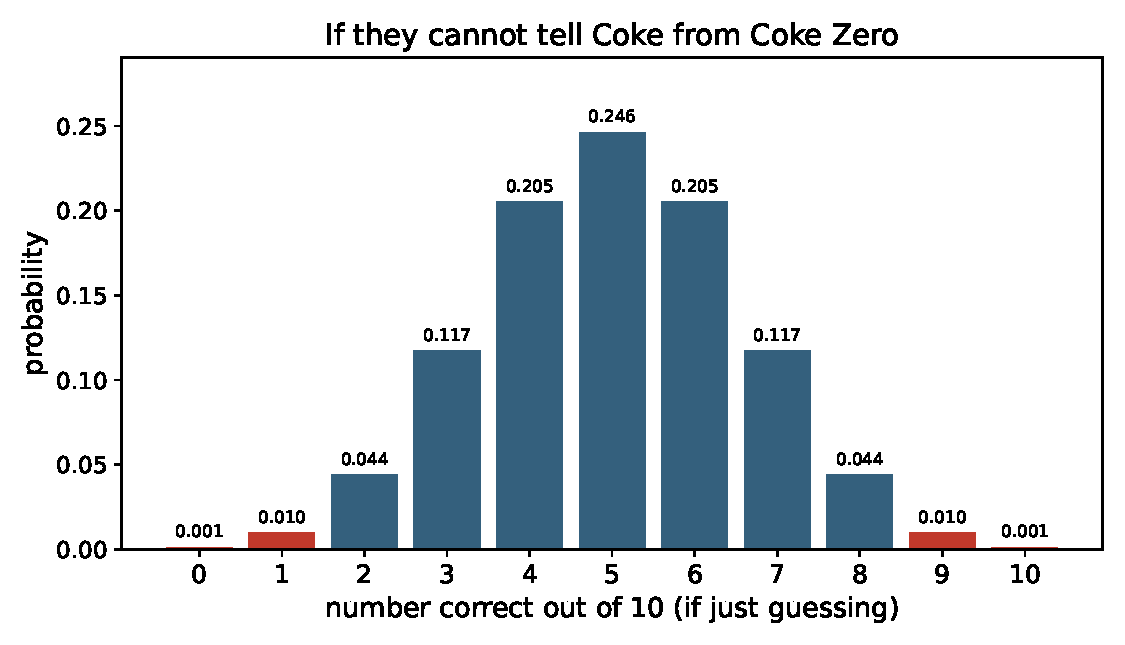
\includegraphics[width=\textwidth]{fig_binom10.pdf}
\end{column}
\begin{column}{0.34\textwidth}
\small
If they're only guessing, the number they get right follows a simple coin-flip pattern
(a Binomial with $n=10$).
\vspace{0.6em}

\textbf{By luck alone:}
\begin{itemize}
  \item $\ge 8$ right: \textbf{5.5\%}
  \item $\ge 9$ right: \textbf{1.1\%}
  \item all 10: \textbf{0.1\%}
\end{itemize}
\vspace{0.4em}
A score out in the \textcolor{red!70!black}{\textbf{red tail}} is hard to chalk up to luck.
\end{column}
\end{columns}
\end{frame}

\begin{frame}{You just re-ran a famous experiment}
\begin{columns}[T]
\begin{column}{0.6\textwidth}
\begin{itemize}
  \item What we just did has a name. At a 1920s Cambridge tea party, \textbf{Muriel Bristol}
        claimed she could taste whether the milk or the tea was poured into the cup first.
  \item \textbf{Ronald Fisher} did exactly what we did: assume she's guessing, then ask how
        surprising her results would be. (He used 8 cups of tea, we used 10 cups of Coke.)
  \item She got all 8 right, which would happen only about 1.4\% of the time by chance.
\end{itemize}
\end{column}
\begin{column}{0.4\textwidth}
\begin{principle}{the whole idea, in one sentence}
A hypothesis test is just the Coke test. Assume ``they're only guessing,'' then measure how
surprising the data are. Surprising enough, and you start to doubt the guessing story.
\end{principle}
\end{column}
\end{columns}
\end{frame}

\begin{frame}{What this unit gives you}
\begin{columns}[T]
\begin{column}{0.5\textwidth}
\textbf{Things to know}
\begin{itemize}\small
  \item sampling variability and the standard error
  \item the template $(\text{estimate}-\text{null})/\se$
  \item the $t$-statistic and degrees of freedom
  \item what a $p$-value does and does not say
  \item Type I / Type II errors and power
  \item confidence intervals, and the assumptions underneath it all
\end{itemize}
\end{column}
\begin{column}{0.5\textwidth}
\textbf{Mistakes to stop making}
\begin{itemize}\small
  \item ``$p$ is the probability the null is true''
  \item confusing statistical with practical significance
  \item reading ``not significant'' as ``no effect''
  \item trusting a flashy result from a tiny sample
  \item ignoring dependence, multiple testing, and peeking
\end{itemize}
\end{column}
\end{columns}
\vspace{0.5em}
\centering\small
Colors are consistent all semester:
\textcolor{blue!70!black}{\textbf{Principle}} to keep,
\textcolor{green!50!black}{\textbf{In practice}} for a judgment call,
\textcolor{red}{\textbf{Trap}} to avoid.
\end{frame}

% ======================================================================
\section{Mindset}
% ======================================================================
\begin{frame}{The one idea behind all of inference}
\begin{itemize}
  \item You have \textbf{data}. But you care about \textbf{the world}, not the data itself.
  \item Your data is one random draw from a process that could have come out differently. Run
        the study again and you'd get different numbers.
  \item So every statistic you compute (a mean, a difference, a slope) is itself a random
        quantity with its own distribution.
\end{itemize}
\begin{principle}{estimate vs.\ parameter}
The \textbf{parameter} is the true unknown out in the world ($\mu$). The \textbf{estimate}
($\xbar$) is your data's best guess at it. Inference is the study of how far the estimate
might be from the parameter.
\end{principle}
\end{frame}

\begin{frame}{A tale of two coffee shops}
\begin{columns}[T]
\begin{column}{0.58\textwidth}
\begin{itemize}
  \item Shop A: \textbf{4.8} stars from \textbf{12} reviews.
  \item Shop B: \textbf{4.5} stars from \textbf{2{,}000} reviews.
  \item A looks higher, but with only 12 reviews its average is all over the place. A couple
        of friends of the owner can swing it.
  \item B's average barely moves no matter who reviews next.
\end{itemize}
\end{column}
\begin{column}{0.42\textwidth}
\begin{principle}{the moral}
A number without its uncertainty is only half a number. ``How sure are we?'' is the question
this whole module teaches you to answer.
\end{principle}
\end{column}
\end{columns}
\vspace{0.5em}
\onslide<2->{%
\centering\small
\textbf{Now suppose each shop gets one more review, a 0-star:}\\[2pt]
Shop A: $4.8 \rightarrow 4.43$ (a single review drags it down by nearly 0.4).\qquad
Shop B: $4.5 \rightarrow 4.50$ (you can barely see a change).%
}
\end{frame}

\begin{frame}{The point estimate is the easy part}
Three ways to report the same A/B test:
\begin{center}\small
\begin{tabular}{p{0.30\textwidth} p{0.60\textwidth}}
\toprule
``Lift was 2.1\%.'' & A number. Says nothing about whether it is real or how far off it
could be. \\[3pt]
``Lift 2.1\%, $p = 0.03$.'' & Adds whether it is distinguishable from zero, and nothing
else. \\[3pt]
``Lift 2.1\%, 95\% CI $0.2\%$ to $4.0\%$, on 40k users.'' & Says how big, how uncertain, and
lets the reader decide whether it is worth shipping. \\
\bottomrule
\end{tabular}
\end{center}
\vspace{0.3em}
\begin{itemize}
  \item Any tool will hand you the first one. Producing the third takes knowing what the estimate
        would have done on a different sample.
  \item This is the habit that separates people who run analyses from people who are trusted to
        interpret them, and it costs one extra line of output.
\end{itemize}
\begin{principle}{report the range, not just the middle}
A point estimate is a guess. A point estimate with an honest interval is a finding.
\end{principle}
\end{frame}

\begin{frame}{Sampling distribution and standard error}
\begin{itemize}
  \item Imagine repeating your study thousands of times. The histogram of all those estimates
        is the \textbf{sampling distribution}.
  \item Its spread is the \textbf{standard error} ($\SE$): the typical distance between your
        estimate and the truth.
\end{itemize}
\[
   \SE(\xbar) \;=\; \frac{\sigma}{\sqrt{n}}
   \qquad\Longrightarrow\qquad
   \text{quadruple } n \text{ to cut the noise in half.}
\]
\begin{principle}{SE is the unit of surprise}
A difference only means something relative to the SE. ``The groups differ by 3'' tells you
nothing until you know whether 3 is large or small in SE units.
\end{principle}
\end{frame}

\begin{frame}{The signal-to-noise template (memorize this)}
Almost every test statistic you'll ever meet is the same fraction:
\[
   \text{test statistic}
   \;=\;
   \frac{\text{signal}}{\text{noise}}
   \;=\;
   \frac{\text{estimate} - \text{value under } \Hzero}{\se(\text{estimate})}.
\]
\begin{itemize}
  \item \textbf{Numerator:} how far your estimate is from what the null predicts (the effect).
  \item \textbf{Denominator:} how much your estimate wobbles from sampling alone.
  \item A large statistic means the gap is big compared to the wobble.
\end{itemize}
\vspace{0.2em}
\centering\small
$t$-tests, regression slopes, A/B tests: they're all just $(\text{estimate}-\text{null})/\se$.
\end{frame}

\begin{frame}{Your turn \#1}
\begin{yourturn}{which result is stronger evidence?}
Two studies each test whether a drug changes blood pressure.
\begin{itemize}
  \item \textbf{Study 1:} estimated drop $= 10$, \quad $\se = 8$.
  \item \textbf{Study 2:} estimated drop $= 2$, \qquad $\se = 0.5$.
\end{itemize}
\vspace{0.4em}
Study 1 has the bigger number. Decide which one is stronger evidence of a real effect, then
practice explaining your reasoning to a neighbor for 60 seconds.
\end{yourturn}
\end{frame}

\begin{frame}{Your turn \#1: answer}
\[
   \text{Study 1: } t = \tfrac{10}{8} = 1.25
   \qquad\qquad
   \text{Study 2: } t = \tfrac{2}{0.5} = 4.0
\]
\begin{itemize}
  \item \textbf{Study 2} is far stronger evidence, even though its effect estimate is smaller.
  \item The raw effect (10 vs 2) is a red herring. What matters is the effect compared to its
        noise.
\end{itemize}
\begin{principle}{the lesson}
Never judge an estimate by its size alone. Always ask: compared to what? The answer is its
standard error.
\end{principle}
\end{frame}

% ======================================================================
\section{The t-statistic}
% ======================================================================
\begin{frame}{What a $t$-statistic actually is}
The one-sample $t$-statistic is just the template with the mean plugged in:
\[
   t \;=\; \frac{\xbar - \mu_0}{s/\sqrt{n}},
   \qquad \text{df} = n-1 .
\]
For comparing two groups (the workhorse of A/B testing):
\[
   t \;=\; \frac{\xbar_A - \xbar_B}{\se(\xbar_A - \xbar_B)} .
\]
\begin{itemize}
  \item It's a standardized distance: how many standard errors is my estimate from the null
        value?
  \item $|t|\approx 2$ is the folklore threshold for ``notable,'' and folklore is where
        folklore is where the traps live.
\end{itemize}
\end{frame}

% == SECOND LIVE ACTIVITY: two-sample version ==
\begin{frame}{Review: the two-sample $t$-test, all on one page}
\footnotesize
Two independent groups, and you want to know whether their means differ.
\[
t \;=\; \frac{\xbar_A - \xbar_B}{\se(\xbar_A - \xbar_B)},
\qquad
\se(\xbar_A - \xbar_B) \;=\; \sqrt{\frac{s_A^2}{n_A} + \frac{s_B^2}{n_B}} \quad\text{(Welch)} .
\]
Welch's df comes from a formula nobody memorizes; let the software report it. Student's pooled
version assumes equal variances and is the special case, not the default.
\begin{center}
\begin{tabular}{p{0.26\textwidth} p{0.26\textwidth} p{0.32\textwidth}}
\toprule
\textbf{Alternative} & \textbf{Reject $\Hzero$ when} & \textbf{$p$-value} \\
\midrule
$\Hone:\ \mu_A > \mu_B$ & $t > t_{\alpha,\,df}$ & $\Pr(T \ge t)$ \\[3pt]
$\Hone:\ \mu_A < \mu_B$ & $t < -t_{\alpha,\,df}$ & $\Pr(T \le t)$ \\[3pt]
$\Hone:\ \mu_A \neq \mu_B$ & $|t| > t_{\alpha/2,\,df}$ & $2\Pr(T \ge |t|)$ \\
\bottomrule
\end{tabular}
\end{center}
\vspace{0.2em}
\begin{trap}{two designs, two different tests}
If each subject appears in \emph{both} groups (before and after, left hand and right hand), the
observations are not independent. Take the differences per subject and run a \textbf{one-sample}
test on those. Using the unpaired test there throws away the pairing and most of your power.
\end{trap}
\end{frame}

\begin{frame}{Live experiment: now two tasters}
\begin{livedemo}{the two-sample taste test}
Two volunteers, each taking the same \textbf{10-cup} Coke test.
\begin{itemize}
  \item Suppose neither one can really tell the difference, so both are just guessing.
  \item We compare their two scores. How far apart should they land, purely by luck?
\end{itemize}
\end{livedemo}
\vspace{0.2em}
\vspace{0.2em}
\centering\small
If taster A gets 8 and taster B gets 3, is that 5-point gap a real difference in skill, or
just luck? Write down how surprised you'd be.
\end{frame}

\begin{frame}{How far apart two guessers land}
\begin{columns}[c]
\begin{column}{0.64\textwidth}
\centering
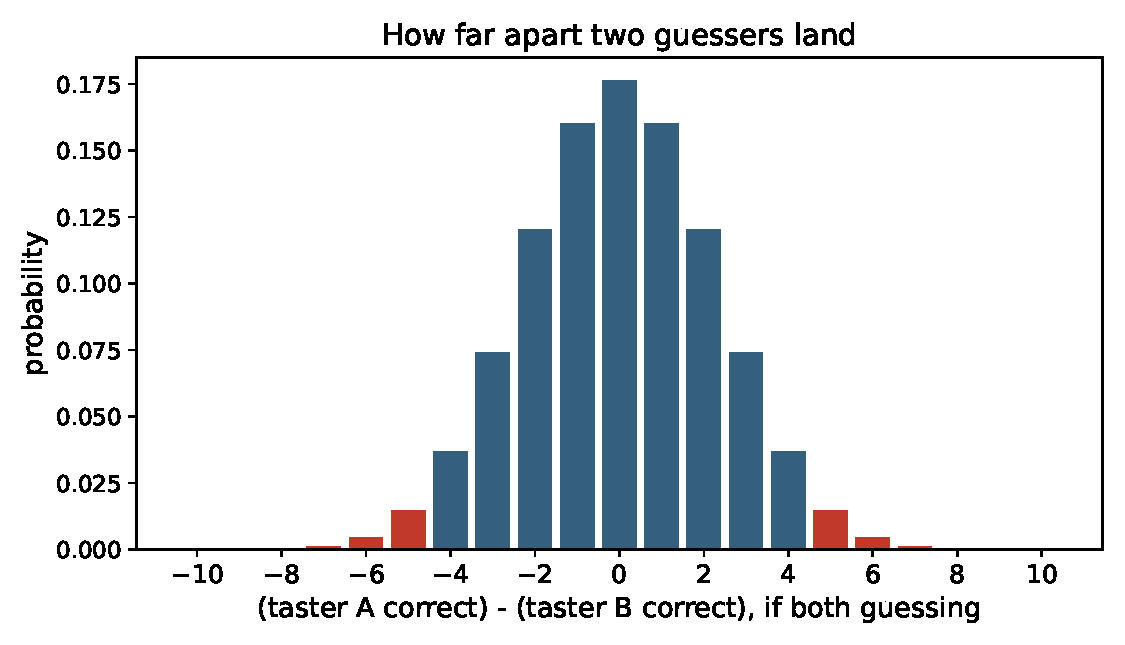
\includegraphics[width=\textwidth]{fig_binom_diff.pdf}
\end{column}
\begin{column}{0.36\textwidth}
\small
The gap between two scores, if \emph{both} are only guessing:
\vspace{0.5em}

\begin{tabular}{lc}
\toprule
gap of $k$ or more & chance \\
\midrule
$\ge 3$ & 0.26 \\
$\ge 4$ & 0.12 \\
$\ge 5$ & \textbf{0.04} \\
$\ge 6$ & 0.01 \\
\bottomrule
\end{tabular}
\vspace{0.5em}

A gap of \textbf{5 or more} happens only \textbf{4\%} of the time by luck. ``How surprising is
the gap?'' is exactly the two-sample $t$ question.
\end{column}
\end{columns}
\end{frame}

\begin{frame}{The $t$-test was invented to brew better beer}
\begin{columns}[T]
\begin{column}{0.6\textwidth}
\begin{itemize}
  \item \textbf{William Gosset} was a chemist at the \textbf{Guinness} brewery, working with
        tiny samples of barley and yeast.
  \item Normal-based ($z$) methods were overconfident at small $n$, so he worked out the
        heavier-tailed correction we now call the $t$-distribution.
  \item Guinness wouldn't let employees publish, so he wrote under the pen name
        \textbf{``Student.''} That's why it's \emph{Student's $t$-test}.
\end{itemize}
\end{column}
\begin{column}{0.4\textwidth}
\begin{principle}{why it matters}
The $t$-test exists precisely because small samples are dangerous. That caution is built into
it, and into half the traps in this module.
\end{principle}
\end{column}
\end{columns}
\end{frame}

\begin{frame}{Why ``$t$'' and not ``$z$''?}
\begin{itemize}
  \item If we \emph{knew} the true noise $\sigma$, the standardized mean would be a standard
        normal, $z$.
  \item We don't. We estimate $\sigma$ with $s$ from the same small sample, which adds a second
        source of uncertainty.
  \item That extra uncertainty gives heavier tails: the $t$-distribution with $n-1$ degrees of
        freedom.
\end{itemize}
\begin{principle}{$t$ turns into $z$ as data pile up}
Small $n$: fat tails, so you need a bigger $t$ to be convinced. Large $n$: $s$ gets close to
$\sigma$ and $t$ becomes $z$. Once $n$ is past about 30 to 60, the difference is cosmetic.
\end{principle}
\end{frame}

\begin{frame}{Degrees of freedom, intuitively}
\begin{itemize}
  \item Degrees of freedom is how many independent pieces of information are left to estimate
        variability after you've spent some estimating the mean.
  \item Spend one on the mean ($\xbar$), and $n-1$ are left for $s$.
  \item Fewer of them means a noisier estimate of the noise, which means fatter tails and more
        caution.
\end{itemize}
\begin{trap}{``df is just $n-1$, who cares''}
With small samples, ignoring df makes you overconfident: you treat a wobbly noise estimate as
if it were exact. The whole point of the $t$-distribution is to stop you.
\end{trap}
\end{frame}

% ======================================================================
\section{p-values}
% ======================================================================
\begin{frame}{The idea so far, in one slide}
\begin{itemize}
  \item Your data is one draw from a process that could have come out differently, so every
        number you compute has a distribution.
  \item The width of that distribution is the \textbf{standard error}.
  \item Every test statistic is
        $\dfrac{\text{estimate} - \text{what the null predicts}}{\text{standard error}}$, which
        asks: is this gap big \emph{compared to how much it naturally wobbles}?
\end{itemize}
\begin{principle}{the question now}
Now we turn that ratio into a probability, and then spend most of this unit on what that
probability does not mean.
\end{principle}
\end{frame}

\begin{frame}{The $p$-value, stated carefully}
\begin{principle}{say it this way, every time}
The $p$-value is the probability of a test statistic \textbf{at least as extreme} as the one
you observed, \textbf{assuming the null hypothesis is true}.
\[
   p \;=\; \Pr\big(\,|T| \ge |t_{\text{obs}}| \;\big|\; \Hzero \text{ true}\,\big).
\]
\end{principle}
\begin{itemize}
  \item \textbf{You already computed one.} In the Coke test, ``$\Pr(\ge 8 \text{ right} \mid
        \text{guessing}) = 5.5\%$'' is a $p$-value.
  \item A small $p$ says ``data like mine would be surprising if the null were true.'' That's
        all it says.
\end{itemize}
\end{frame}

\begin{frame}{What a $p$-value is \emph{not}}
\begin{trap}{the five classic misreadings}
\begin{enumerate}
  \item It is not the probability the null is true. ($p \ne \Pr(\Hzero\mid\text{data})$.)
  \item It is not the probability your result happened ``by chance.''
  \item $1-p$ is not the probability the alternative is true.
  \item A smaller $p$ does not mean a bigger or more important effect.
  \item $p > 0.05$ does not mean ``no effect.'' It means ``not enough evidence here.''
\end{enumerate}
\end{trap}
\end{frame}

\begin{frame}{What $p$-values do when nothing is going on}
Run a study where the two groups are genuinely identical, then do it 5{,}000 more times. Plot the
$p$-values you get.
\begin{itemize}
  \item The histogram comes out \textbf{flat}. Under the null the $p$-value is
        \textbf{uniform} on $[0,1]$: every value is equally likely, and a $p$ of 0.03 is exactly
        as likely as a $p$ of 0.83.
  \item So $p < 0.05$ happens in \textbf{5\% of studies where nothing is happening}, by
        construction. That is not a surprising event, it is the definition.
\end{itemize}
\begin{principle}{the 5\% is a budget you chose, not evidence you found}
$\alpha$ is the false-alarm rate you agreed to tolerate before collecting data. A single
significant result is one draw from that budget, which is why twenty tests on nothing produce
about one ``discovery.''
\end{principle}
\centering\small
You will build this histogram yourself in the code companion. It is the fastest way to stop
over-reading a small $p$.
\end{frame}

\begin{frame}{What actually drives a $p$-value}
Rewrite the two-group $t$ and you can see what's inside it:
\[
   t \;\approx\; \underbrace{\frac{\text{effect size}}{\sigma}}_{\text{standardized signal}}
   \;\times\; \underbrace{\sqrt{\tfrac{n}{2}}}_{\text{sample size}} .
\]
\begin{itemize}
  \item A $p$-value tangles three things together: the true effect, the noise, and the sample
        size.
  \item Hold the effect fixed and grow $n$: $|t|$ grows like $\sqrt{n}$ and $p$ heads toward 0.
\end{itemize}
\begin{principle}{the headline consequence}
With enough data, almost any effect, however trivial, turns ``statistically significant.''
\end{principle}
\end{frame}

\begin{frame}{Scenario 1: a tiny $p$-value with a trivial effect}
\textbf{Setup.} $n = 5{,}000{,}000$ users. Mean session time differs between two designs by
\textbf{0.4 seconds}, $p < 10^{-8}$.
\begin{itemize}
  \item The $p$-value is tiny because $|t|$ grows with $\sqrt{n}$, not because the effect is
        large.
  \item The effect is 0.4s (trivial?), the CI is maybe $[0.36,0.44]$s (precise and small), and
        the decision really comes down to business value.
\end{itemize}
\begin{practice}{how to answer this}
``It's real, but probably irrelevant. At 5M users we can resolve effects far smaller than
anything worth shipping. Show me the effect size and the CI. Significance alone tells us little
here.''
\end{practice}
\end{frame}

\begin{frame}{Scenario 2: twenty tests, one ``winner''}
\textbf{Setup.} A team tests 20 jelly-bean colors against acne. Nineteen show nothing, then
\emph{green} hits $p = 0.04$, and the headline writes itself.
\begin{itemize}
  \item Under a true null, each test fires falsely 5\% of the time. Across 20 tests, the chance
        of at least one false positive is $1-0.95^{20}\approx 64\%$.
  \item So a lone $p=0.04$ out of 20 is about what pure noise produces.
\end{itemize}
\begin{trap}{multiplicity and $p$-hacking}
Every extra test, segment, or peek inflates the false-positive rate. Correct for it
(Bonferroni, FDR) or decide on the one test that matters ahead of time.
\end{trap}
\end{frame}

\begin{frame}{Your turn \#2}
\begin{yourturn}{practice explaining it}
A clinical trial reports $p = 0.04$. A news article writes:
\vspace{0.4em}
\begin{center}\large
\emph{``There is only a 4\% chance the drug doesn't work.''}
\end{center}
\vspace{0.4em}
True or false? Then turn to a neighbor and practice explaining, in your own words, what
$p=0.04$ really says.
\end{yourturn}
\end{frame}

\begin{frame}{Your turn \#2: answer}
\textbf{False.}
\begin{itemize}
  \item $p=0.04$ is computed \emph{assuming the drug does nothing}. It can't also be the
        probability that the drug does nothing. That would be circular.
  \item The right reading: if the drug truly did nothing, we'd see data this striking only
        about 4\% of the time.
  \item The probability the drug works \emph{given} the data ($\Pr(\Hone\mid\text{data})$) is a
        different quantity, and it needs a prior. That's Bayes, and a later module.
\end{itemize}
\end{frame}

% ======================================================================
\section{Hypothesis tests}
% ======================================================================
\begin{frame}{The hypothesis-testing setup}
\begin{itemize}
  \item \textbf{Null $\Hzero$:} the boring default, like ``no difference'' or ``slope is 0.''
  \item \textbf{Alternative $\Hone$:} what you'd act on, one-sided or two-sided.
  \item \textbf{Level $\alpha$:} the false-alarm risk you accept before seeing data (often 0.05,
        which is a convention, not a law).
  \item \textbf{Decision:} reject $\Hzero$ if $p < \alpha$.
\end{itemize}
\begin{principle}{the courtroom analogy}
$\Hzero$ is ``presumed innocent.'' We either find enough evidence to convict (reject) or we
don't. Failing to convict is not the same as proving innocence.
\end{principle}
\end{frame}

\begin{frame}{Two ways to be wrong}
\begin{center}
\begin{tabular}{l|cc}
\toprule
 & \textbf{$\Hzero$ true} & \textbf{$\Hone$ true} \\
\midrule
\textbf{Reject $\Hzero$}      & Type I error ($\alpha$) & Correct (power $=1-\beta$) \\
\textbf{Fail to reject}       & Correct                 & Type II error ($\beta$) \\
\bottomrule
\end{tabular}
\end{center}
\vspace{0.6em}
\begin{itemize}
  \item \textbf{Type I (false positive):} you ship a change that does nothing.
  \item \textbf{Type II (false negative):} you kill a good idea.
  \item $\alpha$ controls Type I by design. Type II is governed by \textbf{power}.
\end{itemize}
\end{frame}

\begin{frame}{Power: the most under-taught idea}
\begin{principle}{definition}
\textbf{Power} $= 1-\beta = \Pr(\text{reject } \Hzero \mid \Hone \text{ true})$: the chance your
test \emph{catches} an effect that is really there.
\end{principle}
Power goes up with:
\begin{itemize}
  \item a larger true effect
  \item a larger sample size $n$
  \item smaller noise $\sigma$.
\end{itemize}
\begin{trap}{low power distorts, it doesn't just miss (the ``winner's curse'')}
When power is low, the only estimates that clear significance are the ones that got lucky and
large, so ``significant'' effects come out systematically overstated. That's why splashy
small-sample findings so often fail to replicate.
\end{trap}
\end{frame}

\begin{frame}{Your turn \#3}
\begin{yourturn}{is the colleague right?}
A new onboarding flow is tested on \textbf{$n=10$} users. Result: $p = 0.40$.
\vspace{0.5em}
A colleague concludes: \emph{``Proven. The new flow makes no difference.''}
\vspace{0.5em}
Do you agree? What's the first question you ask?
\end{yourturn}
\end{frame}

\begin{frame}{Scenario 3: a non-significant result}
\textbf{Answer to Your turn \#3: no.} ``Not detected'' is not the same as ``not there.''
\begin{itemize}
  \item With $n=10$ the study is badly underpowered: it probably couldn't detect even a large,
        real effect, so $p=0.40$ tells you very little.
  \item First question: what effect \emph{could} this study have detected? Then read the CI.
        Something like $[-3\%, +12\%]$ has not ruled out a big positive effect.
\end{itemize}
\begin{principle}{absence of evidence is not evidence of absence}
A non-significant result with a wide CI is inconclusive, not negative. The honest answer is
``we need more data,'' not ``no effect.''
\end{principle}
\end{frame}

% ======================================================================
\section{CIs and significance}
% ======================================================================
\begin{frame}{Confidence intervals: usually the better answer}
\begin{itemize}
  \item A 95\% CI is the set of null values your data would not reject:
        $\text{estimate} \pm (\text{critical } t)\times\se$.
  \item The connection to tests: a two-sided test rejects $\mu_0$ at level $\alpha$ exactly when
        the $(1-\alpha)$ CI leaves $\mu_0$ out.
\end{itemize}
\begin{principle}{why a CI usually beats a $p$-value}
The CI shows the effect's size and its uncertainty in a single object. ``Lift $+2\%$, 95\% CI
$[-1\%,+5\%]$'' says far more than ``$p=0.21$.''
\end{principle}
\end{frame}

\begin{frame}{Statistical vs.\ practical significance}
\begin{columns}[T]
\begin{column}{0.5\textwidth}
\textbf{Statistical significance}
\begin{itemize}
  \item ``Distinguishable from the null.''
  \item Driven by effect \emph{and} $n$.
  \item A $p$-value question.
\end{itemize}
\end{column}
\begin{column}{0.5\textwidth}
\textbf{Practical significance}
\begin{itemize}
  \item ``Big enough to act on.''
  \item Driven by effect size and cost.
  \item A \emph{business} question.
\end{itemize}
\end{column}
\end{columns}
\vspace{0.6em}
\begin{practice}{the question behind half of all A/B tests}
``2M users, the new button raised clicks by $0.03\%$, $p<10^{-6}$. Ship it?'' The statistics are
settled. The real decision is whether $0.03\%$ is worth the engineering and the risk.
\end{practice}
\end{frame}

\begin{frame}{Scenario 4: the A/B test that was ``peeked''}
\textbf{Setup.} An experiment runs on a live dashboard, and the team ships the moment it crosses
$p < 0.05$.
\begin{itemize}
  \item Testing over and over as data arrive (optional stopping) is multiplicity in disguise,
        and the true false-positive rate climbs well above 5\%.
  \item A pure-noise experiment, watched long enough, will eventually cross 0.05 on its own.
\end{itemize}
\begin{interview}{a standard screening question}
``Peeking breaks the nominal $\alpha$. Either fix the sample size in advance, or use methods
built for monitoring, like sequential or always-valid tests. And separately: is the lift worth
shipping?''
\end{interview}
\end{frame}

% ======================================================================
\section{Assumptions}
% ======================================================================
\begin{frame}{What a $t$-test quietly assumes}
\small
Each assumption is easiest to remember as the thing that breaks it.
\begin{enumerate}
  \item \textbf{Independence.} Every row is its own piece of information.
        \emph{Broken by:} 300 students who sat in 10 study groups and compared answers. That is
        closer to 10 opinions than 300.
  \item \textbf{The \emph{estimate} is roughly normal}, which is not the data being normal.
        \emph{Broken by:} 12 customers with wildly skewed spending. At 500 the average is fine
        even though no individual is.
  \item \textbf{The groups share a spread}, or you use Welch, which does not need it.
        \emph{Broken by:} 2{,}000 long-time users who behave alike against 80 new ones who do not.
  \item \textbf{No single point runs the show.} \emph{Broken by:} 18 purchases, one of them a
        \$45{,}000 tractor.
\end{enumerate}
\begin{principle}{which one to worry about first}
Independence by a wide margin, then outliers and skew at small $n$, then unequal variance, and
last the shape of the raw data.
\end{principle}
\end{frame}

\begin{frame}{What each failure actually does to you}
\begin{center}
\footnotesize
\begin{tabular}{p{0.25\textwidth} p{0.30\textwidth} p{0.33\textwidth}}
\toprule
\textbf{What went wrong} & \textbf{Why it hurts} & \textbf{What you see} \\
\midrule
Rows are related to each other
& Asking someone and then their roommate is not two opinions.
& The SE divides by a $\sqrt{n}$ that is too big, so everything looks more certain than it
is. \\[3pt]
One or two extreme values
& That point moves the mean \emph{and} inflates $s$.
& A result that flips when you delete one row. \\[3pt]
Heavy skew, small $n$
& The average of a few skewed numbers is still skewed.
& A $p$-value that is simply wrong, either way. \\[3pt]
Different spreads, different group sizes
& Pooling forces one spread on two groups that do not share one.
& Student's $t$ claims more certainty than it has. \\
\bottomrule
\end{tabular}
\end{center}
\begin{trap}{the one that never announces itself}
The other three leave fingerprints in a plot. Dependence does not. Only knowing how the data was
collected tells you.
\end{trap}
\end{frame}

\begin{frame}{A checklist for any result you're handed}
Run this on every test statistic someone shows you:
\begin{enumerate}
  \item \textbf{Effect size:} how big is it, in units anyone cares about?
  \item \textbf{Uncertainty:} what's the SE or confidence interval?
  \item \textbf{$n$ and power:} could this $n$ detect a meaningful effect? a meaningless one?
  \item \textbf{Assumptions:} independence? outliers? variance? design?
  \item \textbf{Multiplicity:} how many tests or looks produced this number?
  \item \textbf{Decision:} given the costs, what would you actually do?
\end{enumerate}
\end{frame}

\begin{frame}{Your turn \#4}
\begin{yourturn}{same $n$, same formula, same answer?}
Two researchers each want the average resting heart rate of adults, and each collects
\textbf{1{,}000 readings}.
\begin{itemize}
  \item \textbf{A} measures 1{,}000 different people, once each.
  \item \textbf{B} measures \textbf{5} people, 200 times each.
\end{itemize}
Both report a mean of 68 bpm with $\se = s/\sqrt{1000}$, and both get a very tight interval.
\vspace{0.3em}

With a neighbor: are both of those standard errors believable? If not, whose, and what is that
researcher's real sample size?
\end{yourturn}
\end{frame}

\begin{frame}{Your turn \#4: answer}
\textbf{A is fine. B is not, and B's real sample size is much closer to 5 than to 1{,}000.}
\begin{itemize}
  \item B's 200th reading from person 3 says almost nothing new \emph{about adults}. It says
        something about person 3, who is already in the data.
  \item But the formula does not know that. Every extra row divides $\se = s/\sqrt{n}$ by a little
        more, \textbf{as if new information had arrived}. Almost none did.
  \item Take the extreme case where a person's repeats are identical. Then B really has 5 numbers,
        and the honest denominator is $\sqrt{5}$, not $\sqrt{1000}$. The reported SE is too small
        by a factor of $\sqrt{1000/5} = \sqrt{200} \approx \mathbf{14}$, so $t$ is about
        \textbf{14 times too big}.
  \item Real repeats are not identical, so the truth sits between the two. It sits much nearer the
        bad end.
\end{itemize}
\begin{principle}{count independent observations, not rows}
More rows only buy precision when each one is a fresh draw from the population you care about.
\end{principle}
\end{frame}

\begin{frame}{What to do about it, with what you already have}
\begin{itemize}
  \item \textbf{Ask the question first:} what is \emph{one} independent observation here? A person,
        a store, a week, a classroom? That answer, not the row count, is your $n$.
  \item \textbf{Then collapse to it.} Average each person's 200 readings into one number, and run
        the analysis on those 5 values. You throw away 995 rows and gain an honest answer.
  \item The same move handles the business version: 400{,}000 sessions from 12{,}000 users is far
        closer to 12{,}000 than to 400{,}000. Average to the user, then compare.
\end{itemize}
\begin{trap}{a giant $t$ is not reassurance}
When the unit is wrong, a huge test statistic is the most dangerous output you can get. A $t$ of 31
is then telling you about your denominator, not about the world.
\end{trap}
\end{frame}

\begin{frame}{Scenario 5: significant, but small and skewed}
\textbf{Setup.} $n=18$ per group, revenue data (heavy right skew, one ``whale''), $p=0.02$.
\begin{itemize}
  \item Two red flags collide: a small $n$ (the CLT hasn't rescued normality) and a single
        outlier that can manufacture, or hide, significance.
  \item \textbf{Quick diagnostic:} compare the mean to the median. On symmetric data they nearly
        agree. When the mean sits far above the median, a tail is pulling it, and the mean is no
        longer describing a typical case.
  \item Pressure-test it: does the conclusion survive if you drop that one observation? What if
        you compare medians instead of means, or analyze on a log scale?
\end{itemize}
\begin{practice}{how to answer this}
``I don't trust this $p$ yet. With $n=18$ and a heavy tail, one observation may be doing all the
work. I'd show the result with and without the outlier, and with a robust method.''
\end{practice}
\end{frame}

\begin{frame}{Scenario 6: unequal variances or paired data}
\textbf{Setup.} Group A ($n=2000$, low variance) vs.\ Group B ($n=80$, high variance).
\begin{itemize}
  \item Unequal variances together with unequal $n$ is exactly where Student's $t$ misfires.
        Use \textbf{Welch's $t$}. It is free and it fixes the problem.
  \item Different design: was each user measured before and after? Those two numbers aren't
        independent, so use a \textbf{paired} test on the differences, or you throw away power.
\end{itemize}
\begin{practice}{how to answer this}
``First I'd ask about the design: independent or paired, and are the variances comparable? That
choice, Welch vs.\ Student and paired vs.\ unpaired, changes the answer more than the data do.''
\end{practice}
\end{frame}

% ======================================================================
\section{Consolidate}
% ======================================================================
\begin{frame}{Running a two-group comparison, start to finish}
\small
\begin{enumerate}
  \item \textbf{Write down $\Hzero$, $\Hone$, and $\alpha$ before you look.} One-sided or two-sided is decided here, not later.
  \item \textbf{Check the design.} Independent groups, or the same subjects measured twice? Paired data goes to a one-sample test on the differences.
  \item \textbf{Plot both groups} before any test. Look for skew, outliers, and whether the groups are even comparable.
  \item \textbf{Report $n$, mean, and SD} for each group.
  \item \textbf{Run Welch's test}, which does not assume equal variances: \texttt{stats.ttest\_ind(a, b, equal\_var=False)}.
  \item \textbf{Compute the CI for the difference}, $(\xbar_A-\xbar_B) \pm t^{*}\se$, because that is the number you will actually report.
  \item \textbf{Report all four:} the effect size in real units, the interval, the $p$-value, and $n$.
\end{enumerate}
\end{frame}

\begin{frame}{The traps, all in one place}
\begin{trap}{the ones that bite most often}
\begin{itemize}
  \item ``$p$ is the probability the null is true'' (it isn't).
  \item ``Smaller $p$ means a bigger effect'' (no, $p$ confounds effect, noise, and $n$).
  \item Treating statistical significance as practical importance (different questions).
  \item Reading non-significant as no effect (could be low power, so check the CI).
  \item Trusting a significant estimate from a tiny sample (winner's curse).
  \item Ignoring multiplicity, peeking, and $p$-hacking.
  \item Treating dependent data as independent (silent, deadly, inflates $t$).
  \item Worshiping 0.05 as a cliff instead of reading $p$ as continuous evidence.
\end{itemize}
\end{trap}
\end{frame}

\begin{frame}{Ten questions to be able to answer}
Not to recite. To reason through, out loud, in a couple of sentences each.
\begin{enumerate}\small
  \item Define a $p$-value in one clear sentence, then name three things it is \emph{not}.
  \item 2 million users, a $0.03\%$ lift, $p<10^{-6}$. Ship it?
  \item A result comes back at $p=0.06$. What do you tell a stakeholder?
  \item Your experiment was not significant. Does that mean no effect? How would you check?
  \item You tested twenty features and one was significant. How excited should you be?
  \item Two groups, very different sizes and variances. Which test, and why?
  \item A teammate stops the test the moment $p$ drops below $0.05$. What breaks?
  \item You pooled 400{,}000 sessions across two cities and got $t=31$. Impressed?
  \item When would you rather report a confidence interval than a $p$-value?
  \item A study with 15 observations reports a significant effect. Do you trust its \emph{size}?
\end{enumerate}
\end{frame}

\begin{frame}{Mastery checklist}
You have this unit when you can, from memory:
\begin{itemize}
  \item explain why every estimate has a sampling distribution and an SE
  \item write any test as $(\text{estimate}-\text{null})/\se$ and interpret each part
  \item say precisely what a $t$-statistic, $p$-value, and CI mean, and what they don't
  \item lay out the Type I / Type II / power trade-off and what moves each
  \item separate statistical from practical significance on the spot
  \item name the $t$-test's assumptions in order of fragility, and what to do when each fails
  \item run the six-point checklist on a fresh result and reach a defensible decision
\end{itemize}
\end{frame}

\begin{frame}{A mental model for ``what does this statistic mean?''}
\begin{principle}{the reusable answer structure}
\begin{enumerate}
  \item \textbf{Name the template:} ``this is (estimate $-$ null) over its SE.''
  \item \textbf{Decompose:} is it a real effect, a huge $n$, or tiny noise?
  \item \textbf{Quantify:} ask for the effect size and the confidence interval.
  \item \textbf{Interrogate the design:} independence, outliers, variance, multiplicity, peeking.
  \item \textbf{Decide:} translate it into costs and a recommendation.
\end{enumerate}
\end{principle}
\vspace{0.2em}
\centering
That's how you turn a scary number into a calm, confident answer.
\end{frame}

\begin{frame}{What you should be able to do with software}
\small
Nobody is asking you to memorize syntax. You are expected to know \emph{which} procedure the
question calls for, what to hand it, and what the output means. With an AI assistant open, you
should be able to produce any of these and defend the result.
\begin{center}\footnotesize
\begin{tabular}{p{0.44\textwidth} p{0.46\textwidth}}
\toprule
\textbf{You should be able to} & \textbf{What you would reach for} \\
\midrule
One-sample $t$-test against a claimed value & \texttt{stats.ttest\_1samp} \\
Two independent groups (Welch, the default choice) & \texttt{stats.ttest\_ind(..., equal\_var=False)} \\
Before-and-after on the same subjects & \texttt{stats.ttest\_rel} \\
Confidence interval for a mean or a difference & \texttt{stats.t.ppf} with $s/\sqrt{n}$ \\
Critical value or a $p$-value from $t$ & \texttt{stats.t.ppf}, \texttt{stats.t.sf} \\
Power, and the $n$ you would need & \texttt{statsmodels.stats.power.TTestIndPower} \\
Simulate the null to check any of the above & \texttt{rng.normal}, then loop \\
\bottomrule
\end{tabular}
\end{center}
\vspace{0.2em}
\centering\small
If you cannot say what the output means, the fact that you produced it is worth nothing.
\end{frame}

\begin{frame}{Where we go next}
\begin{itemize}
  \item You now have the template: an estimate, its standard error, and the discipline to ask what
        chance alone would have produced.
  \item \textbf{Unit 2} points that template at a relationship instead of a difference. The
        estimate becomes a \emph{slope}, and almost everything from this unit transfers unchanged.
  \item The rest of Part I builds and stress-tests models. Part II, starting at Unit 7, goes back
        and earns the machinery we are about to use on credit.
\end{itemize}
\begin{principle}{the habit to keep}
Before you explain a result, work out what pure chance would have produced. Most of this course is
that one habit, applied to harder situations.
\end{principle}
\end{frame}

\end{document}
